\documentclass[12pt]{article}
\usepackage[utf8]{inputenc}
\usepackage{amsmath, amssymb}
\usepackage{amsthm}

% Define proposition environment
\newtheorem*{proposition}{Proposition}
\usepackage{geometry}
\usepackage{hyperref}
\usepackage{graphicx}
\usepackage{enumitem}
\usepackage{fancyhdr}

\usepackage[most]{tcolorbox}

\newtcolorbox{defbox}[1][]{%
  enhanced,
  colback=white,
  colframe=black,
  fonttitle=\bfseries,
  title=#1,
  coltitle=black,
  attach boxed title to top left={
    xshift=0.5cm,
    yshift=-2mm,
  },
  boxed title style={
    colframe=white,
    colback=white,
    sharp corners=south,
    boxrule=0pt,
    top=0pt,
    bottom=0pt, 
    width=0.5cm,
    height=0.5cm,
  }
}

% Page layout
\geometry{a4paper, margin=1in}
\pagestyle{fancy}
\fancyhf{}
\setlength{\headheight}{15pt}
\fancyhead[L]{\leftmark}
\fancyhead[R]{\thepage}
\renewcommand{\baselinestretch}{1.2}

\newcommand{\uSigma}{\underline\Sigma}
\newcommand{\usigma}{\underline\sigma}
\newcommand{\tr}{\triangleright}
\newcommand{\tl}{\triangleleft}
\newcommand{\blank}{\sqcup}
\newcommand{\ra}{\rightarrow}
\newcommand{\la}{\leftarrow}
% Title and Author
\title{Computational Complexity}
\author{Manuel Mignogna}
\date{\today}

\begin{document}

\maketitle
\tableofcontents
\newpage

\section{Turing Machine}
\subsection{Definition}
Formally, a Turing Machine is a quadruple $M=(K,\Sigma,\delta,s)$ where: $K$ is a finite set of states, $s\in K$ is the initial state, $\Sigma$ is a finite set of symbols (we say that $\Sigma$ is the alphabet of $M$), $\blank\in\Sigma$ is a special symbol called the blank symbol, $\tr\in\Sigma$ is a special symbol called the first symbol, $\delta$ is a transition function $$\delta : K\times\Sigma
 \to (K\cup\{h,\text{"yes"},\text{"no"}\})\times\Sigma\times\{\la,\ra,-\}$$
We assume that $h$ (the halting state), "yes" (the accepting state), and "no" (the rejecting state), and the cursor directions $\la$ for "left", $\ra$ for "right", and $-$ for "stay", are not in $K\cup\Sigma$.
The function $\delta$ is the "program" of the machine. It specifies, for each combination of current state $q\in K$ and current symbol $\sigma\in\Sigma$, a triple $$\delta(q,\sigma)= (p,\rho,D)$$ where: $p$ is the next state, $\rho$ is the symbol to be written on $\sigma$ and $D\in\{\la,\ra,-\}$  is the direction in which the cursor will move. For $\tr$ we require that, if for states $q$ and $p$, $\delta(q,\tr)=(p,\rho,D)$, then $\rho=\tr$ and $D=\ra$. That is, $\tr$ always directs the cursor to the right, and is never erased.

\subsection{Program execution}
How is the program to start? Initially, the state is $s$. The string is initialized to a $\tr$, followed by a finitely long string $x \in (\Sigma - \{\blank\})^*$. We say that $x$ is the input of the Turing machine. The cursor is pointing to the first symbol, always a $\tr$.

From this initial configuration, the machine takes a step according to $\delta$, changing its state, printing a symbol, and moving the cursor; then it takes another step, and another. Note that, by our requirement on $\delta(p, \tr)$, the string will always start with a $\tr$, and thus the cursor will never "fall off" the left end of the string.

Although the cursor will never fall off the left end, it will often wander off the right end of the string. In this case, we think that the cursor scans a $\blank$, which of course may be overwritten immediately. This is how the string becomes longer—a necessary feature if we wish our machines to perform general computation. The string never becomes shorter.

Since $\delta$ is a completely specified function, and the cursor never falls off the left end, there is only one reason why the machine cannot continue: One of the three halting states $h$, "yes", and "no" has been reached. If this happens, we say that the machine has halted. Furthermore, if state "yes" has been reached, we say the machine accepts its input; if "no" has been reached, then it rejects its input. If a machine halts on input $x$, we can define the output of the machine $M$ on $x$, denoted $M(x)$. If $M$ accepts or rejects $x$, then $M(x) = \text{"yes"}$ or $\text{"no"}$, respectively. Otherwise, if $h$ is reached, then the output is the string of $M$ at the time of halting. Since the computation has gone on for finitely many steps, the string consists of a $\tr$, followed by a finite string $y$, whose last symbol is not a $\blank$, possibly followed by a string of $\blank$s ($y$ could be empty). 

We consider string $y$ to be the output of the computation, and write $M(x) = y$. Naturally, it is possible that $M$ will never halt on input $x$. If this is the case, we write $M(x) = \nearrow$.

\subsection{Configuration}
We can define the operation of a Turing machine formally using the notion of a \textit{configuration}. Intuitively, a configuration contains a complete description of the current state of the computation. Formally, a configuration of $M$ is a triple $(q, w, u)$, where $q \in K$ is a state, and $w, u$ are strings in $\Sigma^*$. 

$w$ is the string to the left of the cursor, including the symbol scanned by the cursor, and $u$ is the string to the right of the cursor, possibly empty. $q$ is the current state.
\subsubsection{Configuration Yields}
We say that configuration $(q, w, u)$ \textit{yields} configuration $(q', w', u')$ in one step, denoted 
$$(q, w, u) \xrightarrow{M} (q', w', u'),$$ 
intuitively if a step of the machine from configuration $(q, w, u)$ results in configuration $(q', w', u')$. Formally, it means that the following holds. 

First, let $\sigma$ be the last symbol of $w$, and suppose that $\delta(q, \sigma) = (p, \rho, D)$. Then we must have that $q' = p$. We have three cases:
If $D = \ra$, then $w'$ is $w$ with its last symbol (which was a $\sigma$) replaced by $\rho$, and the first symbol of $u$ appended to it ($\sqcup$ if $u$ is the empty string); $u'$ is $u$ with the first symbol removed (or, if $u$ was the empty string, $u'$ remains empty).
If $D = \la$, then $w'$ is $w$ with $\sigma$ omitted from its end, and $u'$ is $u$ with $\rho$ attached in the beginning.
Finally, if $D = -$, then $w'$ is $w$ with the ending $\sigma$ replaced by $\rho$, and $u' = u$.

Once we defined the relationship of \textit{yields in one step} among configurations, we can define \textit{yields} to be its transitive closure. That is, we say that configuration $(q, w, u)$ \textit{yields} configuration $(q', w', u')$ in $k$ steps, denoted 
$$(q, w, u) \xrightarrow{M^k} (w', q', u'),$$ 
where $k \geq 0$ is an integer, if there are configurations $(q_i, w_i, u_i)$, $i = 1, \ldots, k + 1$, such that $(q_i, w_i, u_i) \xrightarrow{M} (q_{i+1}, w_{i+1}, u_{i+1})$ for $i = 1, \ldots, k$, $(q_1, w_1, u_1) = (q, w, u)$, and $(q_{k+1}, w_{k+1}, u_{k+1}) = (q', w', u')$. 

Finally, we say that configuration $(q, w, u)$ \textit{yields} configuration $(q', w', u')$, denoted 
$$(q, w, u) \xrightarrow{M^*} (q', w', u'),$$ 
if there is a $k \geq 0$ such that $(q, w, u) \xrightarrow{M^k} (q', w', u')$. 

\subsection{Turing Machine for palindromes}
\begin{figure}[h]
\centering
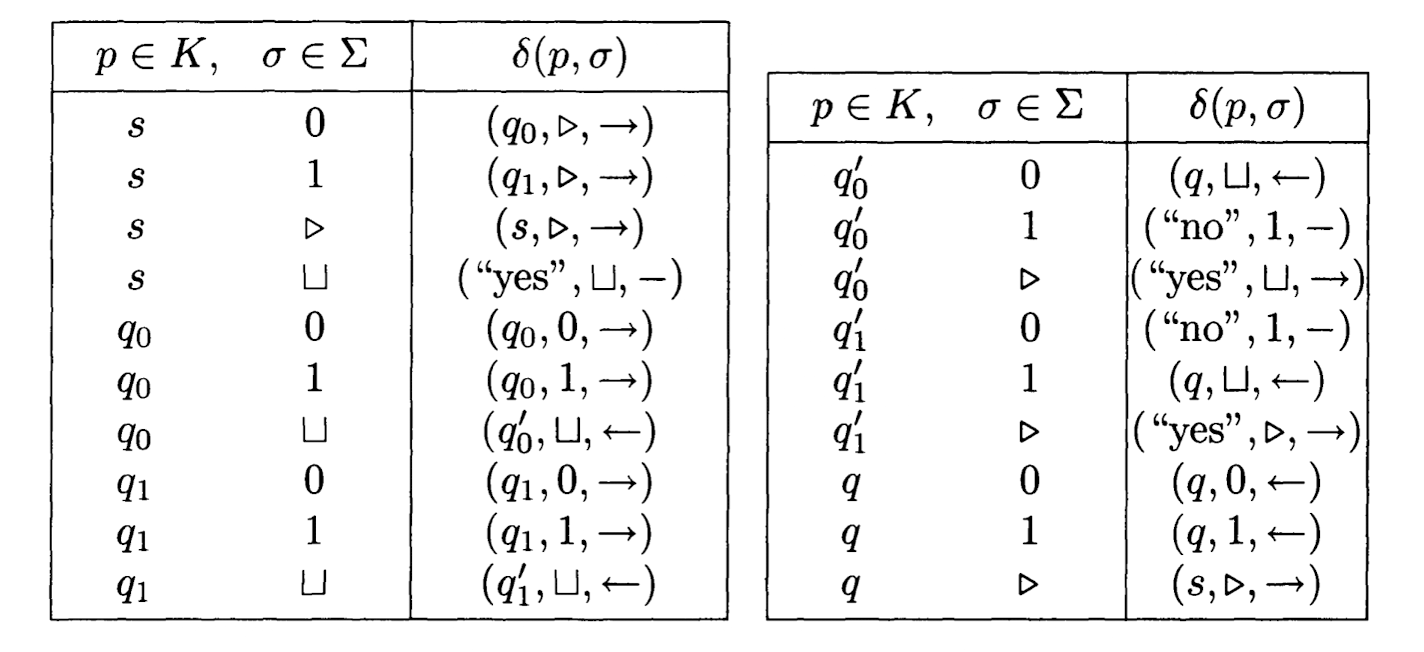
\includegraphics[width=1\textwidth]{img/TM_palindrom.png}
\end{figure}
The machine works as follows: In state $s$, it searches its string for the first symbol of the input. When it finds it, it makes it into a $\tr$ (thus effectively moving the left end of the string inward) and remembers it in its state. By this, we mean that $M$ enters state $q_0$ if the first symbol is a $0$, and state $q_1$ if it is a $1$ (this important capability of Turing machines to remember finite information in their state will be used over and over). $M$ then moves to the right until the first $\sqcup$ is met, and then once to the left to scan the last symbol of the input (now $M$ is in state $q_0'$ or $q_1'$, still remembering the first symbol). If this last symbol agrees with the one remembered, it is replaced with a $\sqcup$ (so that the string implodes on the right as well). Then the rightmost $\tr$ is found using a new state $q$, and then the process is repeated. Notice that, as the two boundaries of the string (a $\tr$ on the left, a $\sqcup$ on the right) have "marched inwards," the string left is precisely the string that remains to be shown a palindrome. If at some point the last symbol is different from the first symbol as remembered by the machine, then the string is not a palindrome, and we reach state "no". If we end up with the empty string (or we fail to find the last symbol, which means that the string was a single symbol) we express our approval by "yes".
\\
On input $0010$, the following configurations, among others, will be yielded:
$$
(s, \tr, 0010) \xrightarrow{M^5} (q_0, \tr 010 \sqcup, \epsilon) \xrightarrow{M} (q_0', \tr 010, \sqcup) \xrightarrow{M} (q, \tr 01, 01 \sqcup) \xrightarrow{M} (s, \tr 0, 1 \sqcup) \xrightarrow{M}$$
$$ (q_0, \tr \tr, 1 \sqcup) \xrightarrow{M^2} (q_0, \tr \tr 1, \sqcup) \xrightarrow{M} (q_0', \tr \tr, \sqcup) \xrightarrow{M} (\text{"no"}, \tr \tr \sqcup, \sqcup).
$$
\\
On input $101$, the computation is as follows:
$$
(s, \tr, 101) \xrightarrow{M^3} (q_1, \tr 01, \sqcup) \xrightarrow{M} (q, \tr 0, 01 \sqcup) \xrightarrow{M} (s, \tr 0, \sqcup) \xrightarrow{M} $$
$$(q_0, \tr \tr, \sqcup) \xrightarrow{M} (q_0', \tr \tr, \sqcup) \xrightarrow{M} (\text{"yes"}, \tr \tr, \sqcup).
$$
\\
On input $\epsilon$ (the shortest palindrome in the world), here is the computation:
$$
(s, \tr, \epsilon) \xrightarrow{M} (s, \tr \sqcup, \epsilon) \xrightarrow{M} (\text{"yes"}, \tr \sqcup, \epsilon).
$$

\subsection{Turing Machines as Algorithms}
\begin{defbox}[Recursive Language]
Let $L \subset (\Sigma - \{\sqcup\})^*$ be a language, that is, a set of strings of symbols. Let $M$ be a Turing machine such that, for any string $x \in (\Sigma - \{\sqcup\})^*$:
If $x \in L$, then $M(x) = \text{"yes"}$ (that is, $M$ on input $x$ halts at the "yes" state),
and if $x \notin L$, then $M(x) = \text{"no"}$.

Then we say that $M$ \textit{decides} $L$. If $L$ is decided by some Turing machine $M$, then $L$ is called a \textit{recursive language}. For example, palindromes over $\{0,1\}^*$ constitute a recursive language decided by machine $M$ defined previously.

We say that $M$ simply \textit{accepts} $L$ whenever, for any string $x \in (\Sigma - \{\sqcup\})^*$:
If $x \in L$, then $M(x) = \text{"yes"}$;
however, if $x \notin L$, then $M(x) = \nearrow$.

If $L$ is accepted by some Turing machine $M$, then $L$ is called \textit{recursively enumerable}.
\end{defbox}

\begin{defbox}
\begin{proposition}
    If $L$ is recursive, then it is recursively enumerable.
\end{proposition}
\begin{proof}
    Suppose that there is a Turing machine $M$ that decides $L$. We shall construct from $M$ a Turing machine $M'$ that \textit{accepts} $L$, as follows: $M'$ behaves exactly like $M$. Except that, whenever $M$ is about to halt and enter state "no", $M'$ moves to the right forever, and never halts.
\end{proof}
\end{defbox}

\begin{defbox}[Recursive Function]
     We shall not only deal with the decision and acceptance of languages, but also occasionally with the \textit{computation of string functions}. Suppose that $f$ is a function from $(\Sigma - \{\sqcup\})^*$ to $\Sigma^*$, and let $M$ be a Turing machine with alphabet $\Sigma$. We say that $M$ \textit{computes} $f$ if, for any string $x \in (\Sigma - \{\sqcup\})^*$, $M(x) = f(x)$. If such an $M$ exists, $f$ is called a \textit{recursive function}.
\end{defbox}

\subsection{Problems encoding}
Thus, Turing machines can be thought of as algorithms for solving string-related problems. But how about our original project, to develop a notation for algorithms capable of attacking problems like those identified in the previous chapter, whose instances are mathematical objects such as graphs, networks, and numbers? 

To solve such a problem by a Turing machine, we must decide how to \textit{represent by a string} an instance of the problem. Once we have fixed this representation, an algorithm for a decision problem is simply a Turing machine that decides the corresponding language. That is, it accepts if the input represents a "yes" instance of the problem, and rejects otherwise. Similarly, problems that require more complex output, such as \textsc{Max Flow}, are solved by the Turing machine that computes the appropriate function from strings to strings (where the output is similarly represented as a string).

It should be clear that this proposal is quite general. Any "finite" mathematical object of interest can be represented by a finite string over an appropriate alphabet. For example:
- Elements of finite sets, such as the nodes of a graph, can be represented as integers in binary.
- Pairs and $k$-tuples of simpler mathematical objects are represented by using parentheses and commas.
- Finite sets of simpler objects are represented by using set brackets, and so on.

Or, perhaps, a graph can be represented by its \textit{adjacency matrix}, which in turn can be arranged as a string, with rows separated by some special symbol such as `;`.

There is a wide range of acceptable representations of integers, finite sets, graphs, and other such elementary objects. They may differ a lot in form and succinctness. \textit{However, all acceptable encodings are related polynomially.} That is, if $A$ and $B$ are both "reasonable" representations of the same set of instances, and representation $A$ of an instance is a string with $n$ symbols, then representation $B$ of the same instance has length at most $p(n)$, for some polynomial $p$. For example, representing a graph with no isolated points by its adjacency matrix is at most quadratically more wasteful than representing it by an adjacency list.

Representing numbers in unary, instead of binary or decimal, is about the only possible slip in this regard. Obviously, the unary representation (in which, for example, number 14 is "IIIIIIIIIIIIII") requires exponentially more symbols than the binary representation. As a result, the complexity of an algorithm, measured as a function of the length of the input of the Turing machine, may seem deceptively favorable.

\newpage
\section{Multi-tape Turing Machine}
\begin{defbox}[Definition of Multi-tape Turing Machine]
    A \textit{$k$-string Turing machine}, where $k \geq 1$ is an integer, is a quadruple $M = (K, \Sigma, \delta, s)$, where $K$, $\Sigma$, and $s$ are exactly as in ordinary Turing machines. $\delta$ is a program that must reflect the complexities of multiple strings. Intuitively, $\delta$ decides the next state as before, but also decides \textit{for each string} the symbol overwritten, and the direction of cursor motion by looking at the current state and the current symbol \textit{at each string}. 
    
    Formally, $\delta$ is a function from $K \times \Sigma^k$ to 
    \[
    (K \cup \{h, \text{"yes"}, \text{"no"}\}) \times (\Sigma \times \{\leftarrow, \rightarrow, -\})^k.
    \]
    Intuitively, $\delta(q, \sigma_1, \ldots, \sigma_k) = (p, \rho_1, D_1, \ldots, \rho_k, D_k)$ means that, if $M$ is in state $q$, the cursor of the first string is scanning a $\sigma_1$, that of the second a $\sigma_2$, and so on, then the next state will be $p$, the first cursor will write $\rho_1$ and move in the direction indicated by $D_1$, and so on for the other cursors. 
    
    $\tr$ still cannot be overwritten or passed on to the left: If $\sigma_i = \tr$, then $\rho_i = \tr$ and $D_i = \rightarrow$. Initially, all strings start with a $\tr$; the first string also contains the input. The outcome of the computation of a $k$-string machine $M$ on input $x$ is as with ordinary machines, with one difference: In the case of machines that compute functions, the output can be read from the \textit{last ($k$th) string} when the machine halts.
\end{defbox}

\subsection{2-tape Turing Machine for palindromes}
  \begin{figure}[h]
    \centering
    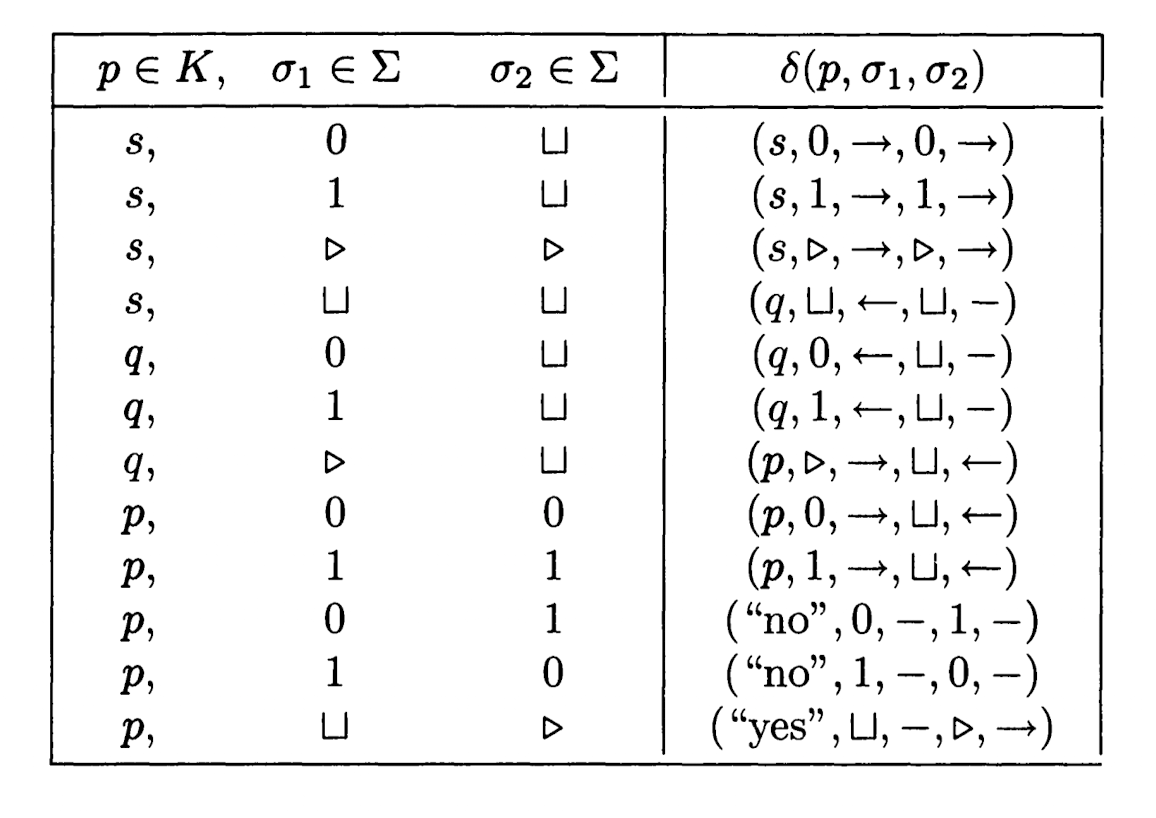
\includegraphics[width=0.8\textwidth]{img/2kTM_palindrom.png}
  \end{figure}
  We can decide palindromes more efficiently with a 2-tape Turing machine. This machine starts by copying its input in the second string. Next,it positions the cursor of the first string at the first symbol of the input, and the cursor of the second string at the last symbol of the copy. Then, it moves the two cursors in opposite directions, checking that the two symbols under them are identical at all steps, at the same time erasing the copy.
  

\subsection{Configuration of a Multi-tape Turing Machine}

A configuration of a $k$-string Turing machine is defined analogously with ordinary Turing machines. It is a $(2k + 1)$-tuple $(q, w_1, u_1, \ldots, w_k, u_k)$, where $q$ is the current state, the $i$th string reads $w_i u_i$, and the last symbol of $w_i$ is holding the $i$th cursor. We say that 
$(q, w_1, u_1, \ldots, w_k, u_k) \text{ yields in one step } (q', w_1', u_1', \ldots, w_k', u_k')$ denoted 
$$(q, w_1, u_1, \ldots, w_k, u_k) \xrightarrow{M} (q', w_1', u_1', \ldots, w_k', u_k')$$
if the following is true. 

First, suppose that $\sigma_i$ is the last symbol of $w_i$, for $i = 1, \ldots, k$, and suppose that 
\[
\delta(q, \sigma_1, \ldots, \sigma_k) = (p, \rho_1, D_1, \ldots, \rho_k, D_k).
\]
Then, for $i = 1, \ldots, k$ we have the following:
- If $D_i = \rightarrow$, then $w_i'$ is $w_i$ with its last symbol (which was a $\sigma_i$) replaced by $\rho_i$, and the first symbol of $u_i$ appended to it ($\sqcup$ if $u_i$ is the empty string); $u_i'$ is $u_i$ with the first symbol removed (or, if $u_i$ was the empty string, $u_i'$ remains empty).
- If $D_i = \leftarrow$, then $w_i'$ is $w_i$ with $\sigma_i$ omitted from its end, and $u_i'$ is $u_i$ with $\rho_i$ attached in the beginning.
- Finally, if $D_i = -$, then $w_i'$ is $w_i$ with the ending $\sigma_i$ replaced by $\rho_i$, and $u_i' = u_i$.

In other words, the conditions for yielding in single-string Turing machines must hold at each string. The relations ``yields in $n$ steps'' and plain ``yields'' are defined analogously with ordinary Turing machines.

A $k$-string Turing machine starts its computation on input $x$ with the configuration 
\[
(s, \tr, x, \tr, \epsilon, \ldots, \tr, \epsilon);
\]
that is, the input is the first string, and all strings start with an $\tr$. If 
\[
(s, \tr, x, \tr, \epsilon, \ldots, \tr, \epsilon) \xrightarrow{M^*} (\text{"yes"}, w_1, u_1, \ldots, w_k, u_k),
\]
for some strings $w_1, u_1, \ldots, u_k$, then we say that $M(x) = \text{"yes"}$; if 
\[
(s, \tr, x, \tr, \epsilon, \ldots, \tr, \epsilon) \xrightarrow{M^*} (\text{"no"}, w_1, u_1, \ldots, w_k, u_k),
\]
then we say that $M(x) = \text{"no"}$. Finally, if the machine halts at configuration $(h, w_1, u_1, \ldots, w_k, u_k)$, then $M(x) = y$, where $y$ is $w_k u_k$ with the leading $\triangleright$ and all trailing $\sqcup$s removed. That is, if $M$ halts at state $h$ (the state that signals the output is ready), the output of the computation is contained in the last string. 

Notice that, by these conventions, an ordinary Turing machine is indeed a $k$-string Turing machine with $k = 1$. Also, once the meaning of $M(x)$ has been defined, we can simply extend to multistream Turing machines the definitions of function computation, and language decision and acceptance of the previous section.

\subsection{TIME class}
\begin{defbox}[TIME class]
  We shall use the multistreaming model of the Turing machine as the basis of our notion of the time expended by Turing machine computations (for space we shall need a minor modification introduced later in this chapter).

  If for a $k$-string Turing machine $M$ and input $x$ we have 
  \[
  (s, \triangleright, x, \triangleright, \epsilon, \ldots, \triangleright, \epsilon) \xrightarrow{M^t} (H, w_1, u_1, \ldots, w_k, u_k)
  \]
  for some $H \in \{h, \text{"yes"}, \text{"no"}\}$, then the time required by $M$ on input $x$ is $t$. That is, the time required is simply the number of steps to halting. If $M(x) = \nearrow$, then the time required by $M$ on $x$ is thought to be $\infty$ (this will rarely be the case in this book).
  
  Defining the time requirements of a single computation is only the start. What we really need is a notion that reflects our interest in solving any instance of a problem, instead of isolated instances. Recall that the performance of algorithms in the previous chapter was characterized by the amount of time and space required on instances of ``size'' $n$, when these amounts were expressed as a function of $n$. For graphs, we used the number of nodes as a measure of ``size.'' For strings, the natural measure of size is the length of the string. Accordingly, let $f$ be a function from the nonnegative integers to the nonnegative integers. We say that machine $M$ operates within time $f(n)$ if, for any input string $x$, the time required by $M$ on $x$ is at most $f(|x|)$ (by $|x|$ we denote the \textit{length} of string $x$). Function $f(n)$ is a time bound for $M$.
  
  Suppose now that a language $L \subset (\Sigma - \{\sqcup\})^*$ is decided by a multistream Turing machine operating in time $f(n)$. We say that $L \in \text{TIME}(f(n))$. That is, $\text{TIME}(f(n))$ is a set of languages. It contains exactly those languages that can be decided by Turing machines with multiple strings operating within the time bound $f(n)$.
  \textbf{TIME}$(f(n))$ is what we call a \textit{complexity class}. It is a set of languages (hopefully, including many that represent important decision problems). The property shared by these languages is that they can all be decided within some specified bound on some aspect of their performance (time, soon space, and later others). Complexity classes, and their relationship with the problems they contain, are the main objects of study in this book.
\end{defbox}


\subsection{Speed up Multi-tape}

\begin{defbox}[Theorem (Speed up Multi-tape)]
  Given any $k$-string Turing Machine $M$ operating within time $f(n)$, we can construct single string Turing Machine $M'$ operating within time $O(f(n)^2)$ and such that, for any input $x$, $M(x)=M'(x)$
\end{defbox}
\begin{proof}
Suppose that $M=(K,\Sigma,\delta,s)$; We shall describe $M'=(K',\Sigma',\delta',s)$. 
  $M'$ single string must "simulate" the $k$ strings of $M$. 
  
  One way to do this would be to maintain in $M'$'s string the concatenation of the strings of $M$ (without, of course the $\tr_s$ that would come in the way of going back and forth in the string). We must also "remember" the position of each cursor, as well as the current right end of each string.
  To accomplish all this, we let $$\Sigma'=\Sigma'\cup\uSigma\cup\{\tr',\tl\}$$ Here $\uSigma=\{\usigma:\sigma\in\Sigma\}$ is a set of cursor versions of the symbol in $\Sigma$.
  $\tr'$ is a new version of $\tr$ which can be passed over to the left, and $\tl$ marks the right end of a string.
  
  Thus, any configuration $(q,w_1,u_1,\dots,w_k,u_k)$ can be simulated by the configurations of $M'$ $(q,\tr,w_1'u_1\tl w_2'u_2\tl\dots w_k'u_k\tl\tl)$. Here $w_i'$ is $w_i$ with the leading $\triangleright$ replaced by $\triangleright'$, and the last symbol $\sigma_i$ by $\underline{\sigma_i}$. The last two $\triangleleft$s signal the end of $M'$'s string.

  For the simulation to begin, $M'$ has simply to shift its input one position to the right, precede it with a $\triangleright'$, and write the string 
  $ \triangleleft (\triangleright' \triangleleft)^{k-1} \triangleleft$
  after its input. This can be easily accomplished by adding to the states of $M'$ $2k + 2$ new states, whose sole purpose is to perform this writing.
  
  To simulate a move of $M$, $M'$ scans twice its string from left to right and back. In the first scan, $M'$ gathers information concerning the $k$ currently scanned symbols in $M$: They are the $k$ underlined symbols encountered. To do this ``remembering,'' $M'$ must contain new states, each of which corresponds to a particular combination of a state of $M$ and of a $k$-tuple of symbols of $M$.
  
  Based on its state at the end of the first scan, $M'$ knows what changes need to be performed on the string to reflect changes in the strings of $M$ at the move being simulated. Then $M'$ scans its string again from left to right, stopping at each underlined symbol to rewrite one or two symbols nearby, in a manner that reflects the symbols overwritten and the cursor motions of $M$ at this string during this move. These updates can be easily performed based on the information available to $M'$.

  There is however one complication: If a cursor scanning the right end of a string needs to move right, we must create space for a new symbol (a $\sqcup$). This is done by first marking the currently scanned $\lhd$ by a special mark, making it $\lhd'$, moving $M'$'s cursor all the way to the $\lhd$ on the right end, and moving all symbols one position to the right, as was done by the Turing machine in Example 2.1. When the $\lhd'$ is encountered, it is moved to the right as a simple $\lhd$, and a $\sqcup$ is overwritten in its old position. Then we go on to implement the changes in the next string of $M$.
  
  The simulation proceeds until $M$ halts. At this point, $M'$ erases all strings of $M$ except the last (so that its output is the same as that of $M$) and halts.
  
  How long does the operation of $M'$ on an input $x$ take? Since $M$ halts within time $f(|x|)$, during its operation none of its strings ever becomes longer than $f(|x|)$ (this is a very basic fact about any reasonable model of computation: It cannot waste more space than time!). Thus the total length of the string of $M'$ is never more than $k(f(|x|) + 1) + 1$ (to account for the $\lhd$s). Simulating a move thus takes at most two traversals of this string from left to right and back ($4k(f(|x|) + 1) + 4$ steps), plus at most $3k(f(|x|) + 1) + 3$ steps per each string of $M$ simulated. The total is $\mathcal{O}(k^2 f(|x|)^2)$, or, since $k$ is fixed and independent of $x$, $\mathcal{O}(f(|x|)^2)$.
\end{proof}

\subsection{Linear Speedup Theorem}
As a result of this theorem, we have that e.g. 
$$\text{if } L\in\textbf{TIME}(150n^2) \text{ then } L\in\textbf{TIME}(n^2 + n +2)$$  
From this we can conclude that, $O()$ is the only significative notation for time complexity.
\begin{defbox}[Linear Speedup Theorem]
  Let $L\in\textbf{TIME}(f(n))$. Then, for any $\epsilon>0$, $L\in\textbf{TIME}(f'(n))$, where $$f'(n) = \epsilon f(n)+n+2$$ 
\end{defbox}

\subsection{Space Bounds}
At first it seems straightforward to define the space used by the computation 
\[
(s, \triangleright, \epsilon, \ldots, \triangleright, \epsilon) \xrightarrow{M^*} (H, w_1, u_1, \ldots, w_k, u_k)
\]
of a Turing machine with $k$ strings. Since the strings cannot become shorter in our model, the lengths of the final strings $w_i u_i$, $i = 1, \ldots, k$, capture the amount of storage required by each during the computation. We can either add up these lengths, or take their maximum. There are arguments in favor of both approaches, but we shall cut the discussion short by noting that the two estimates differ by at most $k$, a constant. Let us say for the time being that the space used by the machine $M$ on $x$ is 
\[
\sum_{i=1}^k |w_i u_i|.
\]
It turns out that this estimate represents a serious overcharge. Consider the following example:

\begin{tcolorbox}[colback=white, colframe=black, title=Example]
\textbf{Can we recognize palindromes in space substantially less than $n$?} 

In view of our definition of the space used by a computation, the sum of the lengths of the strings at halting, this is impossible: One of these lengths, namely that of the first string carrying the input, will always be at least $|x| + 1$.

But consider the following 3-string Turing machine that recognizes palindromes: The first string contains the input, and is never overwritten. The machine works in stages. At the $i$th stage the second string contains integer $i$ in binary. During the $i$th stage we try to identify and remember the $i$th symbol of $x$. We do this by initializing the third string to $j = 1$, and then comparing $i$ and $j$. Comparisons of the contents of the two different strings are easy to do by moving the two cursors. If $j < i$, then we increment $j$ in binary (recall the machine in Example 2.2), and advance the first cursor to the right, to inspect the next input symbol. If $i = j$ we remember in our state the currently scanned symbol of the input, we reinitialize $j$ to 1, and try to identify the $i$th from the last symbol of $x$. This is done much in the same way, with the first cursor now marching from right to left instead from left to right.

If the two symbols are unequal, we halt with ``no''. If they are equal, we increment $i$ by one, and begin the next stage. If, finally, during a stage, the alleged $i$th symbol of $x$ turns out to be a $\sqcup$, this means that $i > n$, and the input is a palindrome. We halt with a ``yes''.
\end{tcolorbox}

\textbf{What space is needed for the operation of this machine?} It seems fair to assess that the space used up by this machine is $\mathcal{O}(\log n)$. The machine surely looks at the input (computation would be impossible otherwise) \textit{but in a read-only fashion}. There is no writing on the first string. The other two strings are kept at most $\log n + 1$ long. \qed

This example leads us to the following definition: Let $k > 2$ be an integer. A \textit{$k$-string Turing machine with input and output} is an ordinary $k$-string Turing machine, with one important restriction on the program $\delta$: Whenever 
\[
\delta(q, \sigma_1, \ldots, \sigma_k) = (p, \rho_1, D_1, \ldots, \rho_k, D_k),
\]
then (a) $\rho_1 = \sigma_1$, and (b) $D_k \neq \leftarrow$. Furthermore, (c) if $\sigma_1 = \sqcup$, then $D_1 = \leftarrow$. 

Requirement (a) says that at each move, the symbol ``written'' on the first string is always the same as the old symbol, and hence the machine effectively has a read-only input string. Requirement (b) states that in the last (output) string the cursor never moves to the left, and hence the output string is effectively write-only. Finally, (c) guarantees that the cursor of the input string does not wander off into the $\sqcup$s after the end of the input. It is a useful technical requirement, but not necessary.

These restrictions lead to an accurate definition of space requirements, without ``overcharging'' the computation for reading the input and for providing output, that is, for functions involving no ``remembering'' of earlier results of the computation. With these restrictions we shall be able to study space bounds smaller than $n$. However, let us first observe that these restrictions do not change the capabilities of a Turing machine.

\begin{defbox}[Proposition]
  For any $k$-string Turing machine $M$ operating within time bound $f(n)$ there is a $(k+2)$-string Turing machine $M'$ with input and output, which operates within time bound $\mathcal{O}(f(n))$.
\end{defbox}
\begin{proof}
  Machine $M'$ starts by copying its input on the second string, and then simulating the $k$ strings of $M$ on its strings numbered 2 through $k+1$. When $M$ halts, $M'$ copies its output to the $k+2$nd string, and halts.
\end{proof} 

\begin{defbox}[Space Complexity Class]
  Suppose that, for a $k$-string Turing machine $M$ and an input $x$ 
\[
(s, \triangleright, x, \ldots, \triangleright, \epsilon) \xrightarrow{M^*} (H, w_1, u_1, \ldots, w_k, u_k),
\]
where $H \in \{h, \text{"yes"}, \text{"no"}\}$ is a halting state. Then the \textit{space required by $M$ on input $x$} is 
\[
\sum_{i=1}^k |w_i u_i|.
\]
If, however, $M$ is a machine with input and output, then the space required by $M$ on input $x$ is 
\[
\sum_{i=2}^{k-1} |w_i u_i|.
\]
Suppose now that $f$ is a function from $\mathbb{N}$ to $\mathbb{N}$. We say that \textit{Turing machine $M$ operates within space bound $f(n)$} if, for any input $x$, $M$ requires space at most $f(|x|)$.

Finally, let $L$ be a language. We say that $L$ is in the \textit{space complexity class} $\textbf{SPACE}(f(n))$ if there is a Turing machine with input and output that decides $L$ and operates within space bound $f(n)$. For example, palindromes were shown to be in the space complexity class $\textbf{SPACE}(\log n)$. This important space complexity class is usually referred to as $\mathbf{L}$.  
\end{defbox}

\begin{defbox}[Theorem]
  Let $L$ be a language in $\textbf{SPACE}(f(n))$. Then, for any $\epsilon > 0$, 
\[
L \in \textbf{SPACE}(2 + \epsilon f(n)).
\]
\end{defbox}

\section{Nondeterministic Turing Machines}
We shall now break our chain of ``reasonable'' models of computation that can simulate each other with only a polynomial loss of efficiency. We shall introduce an \textit{unrealistic} model of computation, the nondeterministic Turing machine. And we shall show that it can be simulated by our other models with an \textit{exponential} loss of efficiency.
\begin{defbox}[Nondeterministic Turing Machine]
  
  A \textit{nondeterministic Turing machine} is a quadruple $N = (K, \Sigma, \Delta, s)$, much like the ordinary Turing machine. $K$, $\Sigma$, and $s$ are as before. Reflecting the fact that a nondeterministic Turing machine does not have a single, uniquely defined next action, but a choice between several next actions, $\Delta$ is no longer a function from $K \times \Sigma$ to $(K \cup \{h, \text{``yes''}, \text{``no''}\}) \times \Sigma \times \{ \leftarrow, \rightarrow, - \}$, but instead a \textit{relation} $\Delta \subseteq (K \times \Sigma) \times [(K \cup \{h, \text{``yes''}, \text{``no''}\}) \times \Sigma \times \{ \leftarrow, \rightarrow, - \}]$. That is, for each state-symbol combination, there may be \textit{more than one} appropriate next step—or none at all.
\end{defbox}

Nondeterministic Turing machine configurations are exactly like configurations of deterministic machines, but ``yields'' is no longer a function; it is instead a \textit{relation}. We say that configuration $(q, w, u)$ of the nondeterministic Turing machine $N$ \textit{yields} configuration $(q', w', u')$ in one step, denoted
\[
(q, w, u) \stackrel{N}{\rightarrow} (q', w', u'),
\]
intuitively if there is a rule in $\Delta$ that makes this a legal transition. Formally, it means that there is a move $((q, \sigma), (q', \rho, D)) \in \Delta$ such that, either (a) $D = \rightarrow$, and $w'$ is $w$ with its last symbol (which was a $\sigma$) replaced by $\rho$, and the first symbol of $u$ appended to it ($\sqcup$ if $u$ is the empty string), and $u'$ is $u$ with the first symbol removed (or, if $u$ was the empty string, $u'$ remains empty); or (b) $D = \leftarrow$, $w'$ is $w$ with $\sigma$ omitted from its end, and $u'$ is $u$ with $\rho$ attached in the beginning; or finally, (c) $D = -$, $w'$ is $w$ with the ending $\sigma$ replaced by $\rho$, and $u' = u$. $N^k \stackrel{k}{\rightarrow}$ and $N^* \stackrel{*}{\rightarrow}$ can be defined as usual, but $N^k \stackrel{k}{\rightarrow}$ is, once more, no longer a function.

What makes nondeterministic machines so different and powerful is the very weak ``input-output behavior'' we demand of them, that is, our very liberal notion of what it means for such a machine to ``solve a problem.'' Let $L$ be a language and $N$ a nondeterministic Turing machine. We say that $N$ \textit{decides} $L$ if for any $x \in \Sigma^*$, the following is true:
\[
x\in L \iff (s, \tr, x) \stackrel{N^*}{\rightarrow} (\text{"yes"}, w, u)
\]
for some strings $w$ and $u$.

This is the crucial definition that sets nondeterministic machines apart from other models. An input is accepted if there is \textit{some} sequence of nondeterministic choices that results in ``yes.'' Other choices may result in rejection; just one accepting computation is enough. The string is rejected only if no sequence of choices can lead to acceptance.

We say that nondeterministic Turing machine $N$ decides language $L$ \textit{in time} $f(n)$, where $f$ is a function from the nonnegative integers to the nonnegative integers, if $N$ decides $L$, and, moreover for any $x \in \Sigma^*$, if 
\[
(s, \triangleright, x) \stackrel{N^k}{\rightarrow} (q, u, w),
\]
then $k \leq f(|x|)$. That is, we require that $N$, besides deciding $L$, does not have computation paths longer than $f(n)$, where $n$ is the length of the input. Thus, we charge to a nondeterministic computation an amount of time that may be considered unrealistically small. The amount of time charged is the ``depth'' of the computational activity. Obviously, the ``total computational activity'' generated can be exponentially bigger.
\begin{figure}[h]
    \centering
    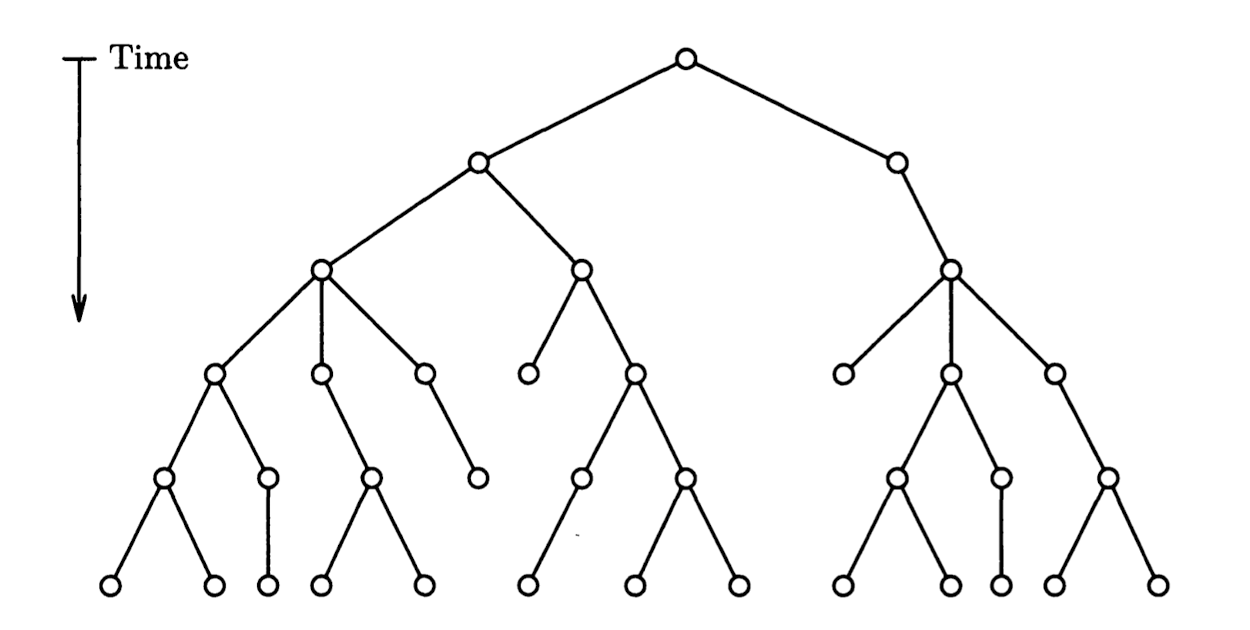
\includegraphics[width=0.8\textwidth]{img/ndc.png}
    \caption{Nondeterministic computation}
    \label{fig:nondeterministic}
\end{figure}
\\
The set of language decided by nondeterministic Turing machines within time $f$ is a new, important kind of complexity class, denoted $\textbf{NTIME}(f(n))$. A most important nondeterministic complexity class is $\textbf{NP}$, the union of all $\textbf{NTIME}(n^k)$. Notice immediately that $\textbf{P}\subseteq\textbf{NP}$; the reason is that deterministic machines from a subclass of the nondeterministic ones: They are precisely those for which the relation $\Delta$ happens to be a function.
\begin{tcolorbox}[colback=white, colframe=black, title=Example]
  Recall that we do not know whether the decision version of the traveling salesman problem, $\text{TSP (D)}$ (recall Section 1.3), is in $\textbf{P}$. However, it is easy to see that $\text{TSP (D)}$ is in $\textbf{NP}$, because it can be decided by a nondeterministic Turing machine in time $\mathcal{O}(n^2)$. This machine, on an input containing a representation of the $\text{TSP}$ instance, goes on to write an arbitrary sequence of symbols, no longer than its input. When this writing stops, the machine goes back and checks to see whether the string written is the representation of a permutation of the cities, and, if so, whether the permutation is a tour with cost $B$ or less. Both tasks can easily be carried out in $\mathcal{O}(n^2)$ time by using a second string (multistring nondeterministic Turing machines are straightforward to define; they can be simulated by single-string ones again with a quadratic slowdown). If the string indeed encodes a tour cheaper than $B$, the machine accepts; otherwise, it rejects (perhaps hoping that another choice of symbols, written at some other branch of the tree in Figure 2.9, will end up accepting).
  
  This machine indeed decides $\text{TSP (D)}$, because it accepts its input if and only if it encodes a ``yes'' instance of $\text{TSP (D)}$. If the input is a ``yes'' instance, this means that there is a tour of the cities with cost $B$ or less. Therefore, there will be a computation of this machine that ``guesses'' precisely this permutation, checks that its cost is indeed below $B$, and thus ends up accepting. It does not matter that other computations of the machine may have guessed very costly tours, or plain nonsense strings, and will therefore reject; a single accepting computation is all that is needed for the machine to accept. Conversely, if there are no tours of cost less than $B$, there is no danger that a computation will accept: All computations will discover that their guess is wrong, and will reject. Thus, according to our convention, the input will be rejected. \qed
  \end{tcolorbox}
  
  It would be remarkable if we could somehow turn this nondeterministic idea into a viable, polynomial-time algorithm for $\text{TSP (D)}$. Unfortunately, at present we know of only exponential general methods for turning a nondeterministic algorithm into a deterministic one. We describe the most obvious such method next.

\begin{defbox}[Theorem (from nondeterministic to deterministic)]
  Suppose that language $L$ is decided by a nondeterministic Turing machine $N$ in time $f(n)$. Then it is decided by a 3-string deterministic Turing machine $M$ in time $\mathcal{O}(cf(n))$, where $c > 1$ is some constant depending on $N$.

Notice that, using complexity class notation, we can restate this result very succinctly:
\[
\textbf{NTIME}(f(n)) \subseteq \bigcup_{c > 1} \textbf{TIME}(cf(n))
\]
\end{defbox}
\begin{proof}
  Let $N = (K, \Sigma, \Delta, s)$. For each $(q, \sigma) \in K \times \Sigma$, consider the set of choices $C_{q,\sigma} = \{(q', \sigma', D) : ((q, \sigma), (q', \sigma', D)) \in \Delta\}$. $C_{q,\sigma}$ is a finite set. Let $d = \max_{q,\sigma} |C_{q,\sigma}|$ (this $d$ could be called the ``degree of nondeterminism'' of $N$), and assume that $d > 1$ (otherwise, the machine is deterministic, and there is nothing to do).

The basic idea for simulating $N$ is this: Any computation of $N$ is a sequence of nondeterministic choices. Now, any sequence of $t$ nondeterministic choices made by $N$ is essentially a sequence of $t$ integers in the range $0, 1, \ldots, d - 1$. The simulating deterministic machine $M$ considers all such sequences of choices, in order of increasing length, and simulates $N$ on each (notice that we cannot simply consider the sequences of length $f(|x|)$, where $x$ is the input, because $M$ must operate with no knowledge of the bound $f(n)$). While considering a sequence $(c_1, c_2, \ldots, c_t)$, $M$ maintains the sequence on its second string. Then $M$ simulates the actions that $N$ would have taken had $N$ taken choice $c_i$ at step $i$ for its first $t$ steps. If these choices would have led $N$ to halting with a ``yes'' (possibili earlier than $t$th step), then $M$ halts with a ``yes'' as well. Otherwise, $M$  proceeds to the next sequence of choices. Generating the next sequence is akin to calculating the next integer in $d$-ary, and can be done easily.
How can $M$ detect that $N$ rejects, with no knowledge of the bound $f(n)$? 
The solution is simple: If $M$ simulates all sequences of choice of a particular 
length $t$, and finds among them \textit{no continuing computation} (that is, all 
computations of length $t$ end with halting, presumably with ``no'' or $h$), then $M$ can 
conclude that $N$ rejects its input.

The time required by $M$ to complete the simulation is bounded from above 
by 
\[
\sum_{t=1}^{f(n)} d^t = O(d^{f(n)+1})
\]
(the number of sequences it needs to go through) times the time required to generate and consider each sequence, and this latter cost is easily seen to be $O(2^{f(n)})$.
\end{proof}
We shall also be very interested in the \textit{space} used by nondeterministic 
Turing machines. To do this correctly for space bounds smaller than linear, we 
shall need to define a \textit{nondeterministic Turing machine with input and output}. 
It is a straightforward task (which we omit) to combine the two extensions of 
Turing machines into one.

Given an $k$-string nondeterministic Turing machine with input and output 
$N = (K, \Sigma, \Delta, s)$, we say that $N$ decides language $L$ within space $f(n)$ if 
$N$ decides $L$ and, moreover, for any $x \in (\Sigma - \{\blank\})^*$, if 
\[
(s, \triangleright, x, \ldots, \triangleright, \epsilon) \xrightarrow{N^*} (q, w_1, u_1, \ldots, w_s, u_s),
\]
then 
\[
\sum_{j=2}^{s-1} |w_j u_j| \leq f(|x|).
\]
That is, we require that $N$ under no circumstances uses space in its ``scratch'' strings greater than function $f$ in the input length. Notice that our definition does not even require $N$ to halt on all computations.

\section{Proper Complexity Functions}
\begin{defbox}[Definition (Proper Complexity Function)]
  Let $f$ be a function from the nonnegative 
integers to the nonnegative integers. We say that $f$ is a \textit{proper complexity 
function} if $f$ is nondecreasing (that is, $f(n+1) \geq f(n)$ for all $n$), and furthermore 
the following is true: There is a $k$-string Turing machine $M_f = (K, \Sigma, \delta, s)$ 
\textit{with input and output} such that, for any integer $n$, and any input $x$ of length 
$n$, 
\[
(s, \triangleright, x, \triangleright, \epsilon, \ldots, \triangleright, \epsilon) 
\xrightarrow{M_f^t} 
(h, x, \triangleright, \sqcup^{j_2}, \triangleright, \sqcup^{j_3}, \ldots, 
\triangleright, \sqcup^{j_{k-1}}, \triangleright, \sqcup^{f(|x|)}),
\]
such that $t = O(n + f(n))$, and the $j_i = O(f(|x|))$ for $i = 2, \ldots, k - 1$, with $t$ and the 
$j_i$'s depending only on $n$. In other words, on input $x$, $M_f$ computes the string 
$\sqcup^{f(|x|)}$, where $\sqcup$ is a ``quasi-blank'' symbol. And, on any input $x$, $M_f$ halts after 
$O(|x| + f(|x|))$ steps and uses $O(f(|x|))$ space besides its input. \qed
\end{defbox}
Using only proper complexity functions we can standardize the behavior of Turing machines.
\begin{defbox}[Precise Turing Machines]
  A Turing Machine (of any type) is \textit{precise} if and only if there exist two proper functions $f$ and $g$ such that, for any input $x$, every computation of $M$ on $x$ halts after exactly $f(|x|)$ steps, and every tape of $M$ beside the input and the output tapes are long exactly $g(|x|)$.
  
\end{defbox}

\begin{defbox}[Theroem (Precise Solutions)]
  Let $M$ be any Turing machine. If $M$ decides a language $L$ in time or space $f(n)$, and $f$ is a proper complexity function, then there exist a precise Turing machine $M'$ that decides $L$ in time or space (respectively) $O(f(n))$.
\end{defbox}
\begin{proof}
  In all four cases (deterministic time, deterministic space, nondeterministic time, or nondeterministic space) the machine $M'$ on input $x$ starts off by simulating the machine $M_f$ associated with the proper function $f$ on $x$, using a new set of strings. After $M_f$'s computation has halted, $M$ uses the output string of $M_f$ as a ``yardstick'' of length $f(|x|)$, to guide its further computation. 

If $f(n)$ is a time bound, then $M'$ simulates $M$ on a different set of strings, \textit{using the yardstick as an ``alarm clock''}. That is, it advances its cursor on the yardstick after the simulation of each step of $M$, and halts if and only if a true blank is encountered, after precisely $f(|x|)$ steps of $M$. If $f(n)$ is a space bound, then $M'$ simulates $M$ on the quasiblanks of $M_f$'s output string. In either case, the machine is precise. 

If $M$ is nondeterministic, then precisely the same amount of time or space is used over all possible computations of $M'$ on $x$, as this amount depends only on the deterministic phase of $M'$ (the simulation of $M_f$). In both cases, the time or space is the time or space consumed by $M_f$, plus that consumed by $M$, and is therefore $\mathcal{O}(f(n))$.

In the case of space-bounded machines, the ``space yardstick'' can be used by $M'$ to also ``count'' steps in an appropriate base representing the size of the alphabet of $M$, and thus $M'$ will never indulge in a meaninglessly long computation. Thus, we can assume that space-bounded machines always halt.
\end{proof}

\begin{defbox}[Theorem (Termination of TM space bounded)]
If $M$ decides $L$ in space $f(n)$, with $f$ being a proper function then exists a Turing machine $M'$ that decides $L$ in space $O(f(n))$ and such that every computation halts.
\end{defbox}
\begin{proof}
  If $M$ works in space $f(n)$, then the set of different configurations in which it can go through is finite. 
  Upper bounder by 
  $$c=|K|\times|\Sigma|^{f(n)}\times (f(n)+1)$$
  If $M$ makes more than $c$ steps, then it must have repeated a configuration and so it must be in a loop. If $M$ doesn't halt in at most $c$ steps we can force termination in "no".
  Proof for 1 tape: concatenates $M_f$ and a simulation of $M$. The last tape of $M_f$ is used as a yardstick. This tape will contain a cell in which we have the symbol representing the current state, it can contain $|K|$ different symbols. Then the next $f(n)$ cells will contain the symbols of $\Sigma$ (represented by an integer in base $|\Sigma|$). The last ($f(n)+1$) cells will be used as an unary representation of the cursor position.
  At every transition of $M$ we increment the counter and if in at most $c$ steps $M$ has not halted, we can force it to halt in "no".
\end{proof}

From this theorem we ca conclude that if the space is finite then the machine will halt. Another important result is that time is exponentially bigger than space. 

\section{Complexity Classes}
\section{Complexity Classes}
\[
\begin{aligned}
    &\text{TIME}(n^k) && = \bigcup_{j > 0} \text{TIME}(n^j)  &&= \textbf{P}, \\
    &\text{NTIME}(n^k) && = \bigcup_{j > 0} \text{NTIME}(n^j)  &&= \textbf{NP}, \\
    &\text{TIME}(2^{n^k}) && = \bigcup_{j > 0} \text{TIME}(2^{n^j})  &&= \textbf{EXP}, \\
    &\text{SPACE}(n^k) && = \bigcup_{j > 0} \text{SPACE}(n^j)  &&= \textbf{PSPACE}, \\
    &\text{NSPACE}(n^k) && = \bigcup_{j > 0} \text{NSPACE}(n^j) && = \textbf{NPSPACE}, \\
    &\text{SPACE}(\log n) &&&& = \textbf{L}, \\
    &\text{NSPACE}(\log n) &&&& = \textbf{NL}.
\end{aligned}
\]
\section{Complementary Complexity Classes}

\end{document}